\documentclass{beamer}

% 中文与英文字体设置(增强稳定性)
\usepackage{xeCJK}
\usepackage{fontspec}

% 主体字体:宋体 + Times + 微软雅黑
\setmainfont{Times New Roman}
\setsansfont{Times New Roman}
\setmonofont{Courier New}

\setCJKmainfont{SimSun}
\setCJKsansfont{Microsoft YaHei}  % 更稳定的无衬线字体,支持加粗

% 标题字体美化
\setbeamerfont{title}{family=\rmfamily}
\setbeamerfont{frametitle}{family=\rmfamily}

% 常用功能包
\usepackage{graphicx}
\usepackage{caption}
\usepackage{listings}
\usepackage{xcolor}
\usepackage{amsmath}
\usepackage{booktabs}
\usepackage{hyperref}
\usepackage{array}
\usepackage{tikz}
\usepackage{ragged2e}

\graphicspath{{image/}}

% 主题与样式设置
\usetheme{Berlin}
\setbeamertemplate{frametitle}[default][center]

% ========= 论文正式信息 =========
\title{基于改进A*算法与自适应权重MPC的\\水面无人艇路径规划研究}
\author{龚家和}
\institute{安徽大学·纽约石溪学院\\应用统计学\\本科毕业论文答辩}
\date{2025年5月9日}

\begin{document}

\begin{frame}[plain]
  \titlepage
\end{frame}

\input{Introduction}
\section{研究背景与问题定义}

\begin{frame}{研究背景(一)技术发展与政策支持}
    \justifying
    随着智能感知、人工智能与控制理论的不断融合,水面无人艇(Unmanned Surface Vehicle, USV)作为具备自主导航、环境感知与远程通信能力的新型平台,正被广泛应用于海洋测绘、环境监测、灾害预警与水面巡逻等任务场景。
    
    \vspace{0.8em}
    USV 拥有低成本、高效率、危险替代性强等突出优势,成为“智能海洋”建设中的关键组成部分。政策层面,《产业结构调整指导目录(2019年)》明确提出支持智能船舶与无人系统的发展,为相关研究提供了良好的政策导向和产业支撑。
    \end{frame}
    
\begin{frame}{研究背景(二)面对挑战与创新动机}
\justifying
尽管 USV 技术发展迅速,但其在实际水域中的路径规划仍面临典型挑战。尤其在存在大量静态非凸障碍物的环境下,传统 A* 算法在建图与启发式设计中未显式考虑“贴边性”信息,其路径往往趋于保守,远离障碍物边缘,导致航行距离延长、效率下降。

\vspace{0.8em}
此外,路径规划与控制器之间缺乏一致性联动,路径在实际跟踪过程中常出现偏差,影响任务可靠性。为此,本研究在 A* 框架中引入“障碍物边界距离感知”机制,通过改进代价函数与启发策略,使路径具备对边界区域的偏好选择特性。同时结合 AN-MPC 控制器进行局部优化,构建感知、规划与控制一体化的多层路径优化体系。
\end{frame}



\begin{frame}{三层次路径规划与控制系统架构}
    \justifying
    本研究围绕 USV 在复杂水域中实现自主、高效、鲁棒路径航行的目标,设计了一套“\textbf{全局路径规划 — 局部轨迹优化 — 动态障碍避障}”三层次路径规划与控制系统。各层功能如下:
    
    \vspace{0.2em}
    \begin{itemize}
      \item \textbf{全局路径规划层(MD-A*)}:基于预设地图信息,构建障碍图模型,引入贴边性启发式与绕行惩罚机制,实现全局高效路径生成。
      
      \item \textbf{局部轨迹优化层(AN-MPC)}:结合 Fossen 简化模型与状态反馈,设计自适应加权 MPC 控制器,实现路径跟踪、能耗与速度平稳性的动态权衡。
      
      \item \textbf{动态障碍避障层(展望)}:引入行为识别与策略切换机制,集成改进型多智能体强化学习方法,提升对动态目标的响应能力与智能调整效果。
    \end{itemize}
    
    \vspace{0.2em}
    系统采用感知-规划-控制闭环架构,支持模块间协同运行与实时动态调度,具备良好的工程扩展性。
    \end{frame}
    
\section{MD-A* 路径规划方法}

% 第一页:方法概述
\begin{frame}{方法概述:改进型 A* 算法(MD-A*)}
    \justifying
    针对传统 A* 算法在水域路径规划中存在路径保守、贴边性差的问题,本文提出融合几何启发式与边界偏好估计的改进方法。

    \vspace{0.8em}
    本研究构建的 \textbf{MD-A*(Modified Distance A*)} 算法在连边建模中引入“绕行代价”和“穿越长度补偿”两类路径代价因素,同时在启发式函数中融入边界结构感知机制,在保持启发式搜索最优性的前提下,引导路径搜索更贴近可行区域边界。

    \vspace{0.5em}
    方法适用于障碍密集、水道不规则等海港场景,具备良好的工程解释性与可行性。
\end{frame}

% 第二页:直观思想演示图
\begin{frame}[plain]{直观思想演示图1}
  \begin{center}
    \includegraphics[width=0.7\textwidth]{Image/MD-Astar思想演示图.png}
    \captionof{figure}{1 “类贴边性”直观思想对比示意图}
  \end{center}
\end{frame}


% 第三页:权重建模
\begin{frame}{权重建模:融合绕行代价与穿越补偿机制}
    \justifying
    综合考虑欧几里得距离、绕行代价及穿越补偿,定义连边 $(P_i, P_j)$ 的权重为:
    \[
    \text{weight}(P_i, P_j) = d_{\text{euclid}}(P_i, P_j) + \lambda d_{\text{绕行}}(P_i, P_j) - \mu d_{\text{穿越}}(P_i, P_j)
    \]
    其中:
    \begin{itemize}
      \item $d_{\text{euclid}}$:欧几里得距离;
      \item $d_{\text{绕行}}$:对绕开障碍最小路径的估算;
      \item $d_{\text{穿越}}$:连线实际穿越障碍物的长度;
      \item $\lambda \geq \mu \geq 1$:分别为绕行代价与穿越补偿的权重。
    \end{itemize}
    特别地,当边未穿越任何障碍时,$d_{\text{绕行}} = d_{\text{穿越}} = 0$,退化为欧几里得权重。
\end{frame}

% 第四页:启发式函数设计与贴边性引导
\begin{frame}{启发式函数设计与贴边性引导}
    \justifying
    为在路径搜索中兼顾启发效率与路径合理性,本文对传统 A* 启发函数进行设计改进:
    \[
    h(n) = d_{\text{euclid}}(n, t) + \min_{(n,m)\in E} \left( d_{\text{绕行}}(n,m) - d_{\text{穿越}}(n,m) \right)
    \]
    其中,第一项衡量当前节点与目标点的基础距离,第二项表达与边界之间的贴边偏好估计。

    \vspace{0.5em}
    \textbf{可接受性}:$h(n)$ 不高估真实代价;
    \textbf{一致性}:满足 $h(n) \leq c(n,m) + h(m)$,确保 A* 的收敛性与最优性。
\end{frame}



\section{AN-MPC 轨迹控制策略}

% === 第1页:AN-MPC方法的理论设计概述 ===
\begin{frame}{AN-MPC 控制理论基础与设计概述}
    \justifying
    为提升 USV 在复杂扰动环境下的局部轨迹优化能力,本文基于简化 Fossen 模型构建 AN-MPC 控制器,通过滚动优化与动态权重机制实现路径跟踪的稳健性与自适应控制。
    
    \vspace{0.6em}
    USV 离散时间状态空间模型为:
    \[
    \boldsymbol{x}(k+1) = f(\boldsymbol{x}(k), \boldsymbol{u}(k)) + \boldsymbol{w}(k)
    \]
    其中:
    \begin{itemize}
        \item $\boldsymbol{x}(k) = [X, Y, \theta, u, v, \omega]^T$ 为状态向量;
        \item $\boldsymbol{u}(k) = [T_{\text{thrust}}, T_{\text{lateral}}, \tau_{\text{yaw}}]^T$ 为控制输入;
        \item $\boldsymbol{w}(k)$ 表示水流扰动。
    \end{itemize}
    状态预测采用数值积分,考虑扰动叠加。
\end{frame}

% === 第2页:直观思想演示图 ===
\begin{frame}[plain]{直观思想演示图2}
  \begin{center}
    \includegraphics[height=0.7\textwidth]{Image/AN-MPC思想演示图.png}
    \captionof{figure}{2 AN-MPC 轨迹优化思想演示图}
  \end{center}
\end{frame}

% === 第3页:USV 简化动力学建模框架 ===
\begin{frame}{USV 简化动力学建模框架}
\justifying
为实现 AN-MPC 控制器在工程上的可部署性,本文在 Fossen 水动力学模型基础上,进行如下简化处理:
\begin{itemize}
    \item 假设惯性矩阵为对角形式;
    \item 阻尼项采用线性速度相关模型;
    \item 外部扰动建模为定速定向的水流矢量;
\end{itemize}

\vspace{0.5em}
简化后的动力学主方程为:
\[
\boldsymbol{M}\nu + \boldsymbol{C}(\nu)\nu + \boldsymbol{D}(\nu')\nu' = \boldsymbol{\tau}
\]
其中:
\begin{itemize}
    \item $\nu = [u, v, \omega]^T$ 为船体速度向量;
    \item $\boldsymbol{\tau} = [T_{\text{thrust}}, T_{\text{lateral}}, \tau_{\text{yaw}}]^T$ 为控制输入;
    \item $\nu' = \nu - \nu_{\text{current}}^{\text{body}}$ 表示相对于水流的扰动速度。
\end{itemize}
\end{frame}

% === 第4页:水流扰动建模与姿态运动学 ===
\begin{frame}{水流扰动建模与姿态运动学}
\scriptsize
\justifying
水流速度在全局坐标系中为:
\[
\nu_{\text{current}}^{\text{global}} = 
\begin{bmatrix}
V \cos \psi \\ V \sin \psi \\ 0
\end{bmatrix}, \quad
\nu_{\text{current}}^{\text{body}} = R(\theta)^T \nu_{\text{current}}^{\text{global}}
\]

\vspace{0.5em}
三大动力学矩阵定义如下:
\[
\boldsymbol{M} =
\begin{bmatrix}
m & 0 & 0 \\
0 & m & 0 \\
0 & 0 & I_z
\end{bmatrix}, \quad
\boldsymbol{C}(\nu) =
\begin{bmatrix}
0 & 0 & -mv \\
0 & 0 & mu \\
mv & -mu & 0
\end{bmatrix}, \quad
\boldsymbol{D}(\nu') =
\begin{bmatrix}
D_u & 0 & 0 \\
0 & D_v & 0 \\
0 & 0 & D_\omega
\end{bmatrix}
\]

\vspace{0.5em}
USV 姿态变化由运动学方程描述:
\[
\begin{bmatrix}
\dot{X} \\ \dot{Y} \\ \dot{\theta}
\end{bmatrix}
= R(\theta)
\begin{bmatrix} u \\ v \\ \omega \end{bmatrix}
\quad \Rightarrow \quad
\nu_{\text{net}} = \nu_{\text{still}} + \nu_{\text{current}}^{\text{global}}
\]
\end{frame}

% === 第5页:AN-MPC控制目标函数与约束建模 ===
\begin{frame}{AN-MPC 控制目标函数与约束建模}
\justifying
每个控制周期内,AN-MPC 控制器求解如下优化问题:
\[
\min_{\boldsymbol{u}(0),\dots,\boldsymbol{u}(N-1)} \sum_{k=0}^{N-1} \left( (\boldsymbol{x}(k) - \boldsymbol{x}_{\text{ref}}(k))^T Q(k)(\boldsymbol{x}(k) - \boldsymbol{x}_{\text{ref}}(k)) + \boldsymbol{u}(k)^T R \boldsymbol{u}(k) \right)
\]
其中:
\begin{itemize}
    \item $Q(k)$ 和 $R$ 为状态误差与控制能耗的权重矩阵;
    \item $N$ 为预测时域长度,$\boldsymbol{x}_{\text{ref}}(k)$ 为参考轨迹;
    \item $Q(k)$ 动态变化,$R$ 为固定矩阵。
\end{itemize}
\end{frame}

% === 第6页:AN-MPC 多目标代价函数设计 ===
\begin{frame}{AN-MPC 多目标代价函数设计}
\justifying
优化目标函数由多个子目标代价组成:
\[
J = J_{\text{error}} + \lambda_1 J_{\text{energy}} + \lambda_2 J_{\text{speed}} + \lambda_3 J_{\text{curvature}} + \lambda_4 J_{\text{current}} + J_{\text{restricted}}
\]

各子目标定义如下:
\begin{itemize}
    \item 轨迹误差项:$J_{\text{error}} = \sum_k (\boldsymbol{x}_k - \boldsymbol{x}_{\text{ref},k})^T Q (\boldsymbol{x}_k - \boldsymbol{x}_{\text{ref},k})$
    \item 能耗项:$J_{\text{energy}} = \sum_k \boldsymbol{u}_k^T R \boldsymbol{u}_k$
    \item 速度平稳性项:$J_{\text{speed}} = \sum_k \left( (u_k - u_0)^2 + (v_k - v_0)^2 \right)$
\end{itemize}
\end{frame}

% === 第7页:AN-MPC 其他代价与补偿项设计 ===
\begin{frame}{AN-MPC 其他代价与补偿项设计}
\justifying
\begin{itemize}
    \item 曲率平滑项:$J_{\text{curvature}} = \sum_k (\theta_{k+1} - \theta_k)^2$
    \item 水流补偿项:
    \[
    J_{\text{current}} = \sum_k (V_{\text{current}} \cos \psi \cdot e_x(k) + V_{\text{current}} \sin \psi \cdot e_y(k))^2
    \]
    \item 禁区惩罚项:$J_{\text{restricted}} = \lambda_5$,若路径进入禁区,否则为 0
\end{itemize}
\end{frame}

% === 第8页:控制输入约束条件 ===
\begin{frame}{控制输入约束条件}
\justifying
控制输入施加如下约束,确保系统稳定与安全性:
\[
\begin{aligned}
T_{\text{thrust,min}} \leq T_{\text{thrust}}(k) &\leq T_{\text{thrust,max}} \\
T_{\text{lateral,min}} \leq T_{\text{lateral}}(k) &\leq T_{\text{lateral,max}} \\
\tau_{\text{yaw,min}} \leq \tau_{\text{yaw}}(k) &\leq \tau_{\text{yaw,max}}
\end{aligned}
\]
\end{frame}

% === 第9页:状态误差权重矩阵 Q(k) 的动态调整机制 ===
\begin{frame}{状态误差权重矩阵 Q(k) 的动态调整机制}
\justifying
每周期根据当前速度状态动态调整误差矩阵 $Q(k)$:
\[
Q(k) = \text{diag} \left(1 + \alpha(u^2 + v^2), 1 + \beta(u^2 + v^2), \frac{1}{1 + \gamma(u^2 + v^2)}, 1, 1, 1 \right)
\]
调整逻辑:
\begin{itemize}
    \item $X,Y$ 方向误差惩罚随速度增大加强;
    \item 航向角误差惩罚随速度增大减弱;
    \item $u,v,\omega$ 权重固定,用于保障稳定性。
\end{itemize}
该机制提升了高速状态下的位置控制精度与低速下的航向灵活性。
\end{frame}

\section{展望:策略切换机制}

% 第一页:动态避障机制设计概述
\begin{frame}{动态障碍物避障机制设计概述}
\justifying
在复杂动态海洋环境中,水面无人艇(USV)经常面临其他船只、漂浮物等动态障碍物干扰。为提升系统在动态环境下的航行安全性与适应能力,本文提出一种结合\textbf{行为识别}与\textbf{策略切换}机制的动态避障方法,并嵌入于整体三层控制架构中。

\vspace{0.5em}
该方法支持智能体根据障碍物运动特性自动选择避障策略:\textbf{可预测运动}使用基于物理建模的轨迹预测与规避方法;\textbf{不可预测运动}则启用深度强化学习(DRL)模块,实现自适应避障与路径优化。
\end{frame}

% 第二页:直观思想演示图
\begin{frame}[plain]{直观思想演示图3}
\begin{center}
    \includegraphics[height=0.7\textwidth]{Image/策略切换演示图.png}
    \captionof{figure}{3 动态避障策略切换思想演示图}
\end{center}
\end{frame}

% 第三页:行为识别与策略切换机制
\begin{frame}{行为识别与策略切换机制}
\justifying
为判断障碍物是否符合固定方向均匀加速模型,系统使用如下二阶差分指标:
\[
\Delta V = \frac{V_{t+1} - V_t}{\Delta t}, \quad \Delta\theta = \frac{\theta_{t+1} - \theta_t}{\Delta t}
\]
当 $|\Delta V|$ 与 $|\Delta\theta|$ 同时低于阈值,认为该障碍物运动可预测,选择物理预测策略;否则启用深度强化学习模块。
\end{frame}

% 第四页:可预测运动下的物理建模策略
\begin{frame}{可预测运动下的物理建模策略}
\justifying
对于判定为可预测的障碍物,其未来轨迹可通过牛顿运动模型近似计算。障碍物在 USV 船体坐标系下的速度与加速度变换为:
\[
\mathbf{V}_b = R(\theta)^T \cdot \mathbf{V}_g, \quad \mathbf{a}_b = R(\theta)^T \cdot \mathbf{a}_g
\]
其中 $R(\theta)$ 为从全局坐标系到船体坐标系的旋转矩阵。

未来位置预测公式:
\[
p_{\text{obs}}(t + \Delta t) = p_{\text{obs}}(t) + \mathbf{V}_b \cdot \Delta t + \frac{1}{2} \mathbf{a}_b (\Delta t)^2
\]
该方法计算负担轻,适用于短时域规避。
\end{frame}

% 第无页:不可预测运动下的强化学习策略
\begin{frame}{不可预测运动下的强化学习策略}
\justifying
若障碍物运动不符合物理模型,USV 启用基于深度强化学习(DRL)的智能避障模块。通过与环境交互,智能体学习最优行为策略以应对高动态性。

奖励函数设计考虑以下目标:
\begin{itemize}
    \item 成功避障率(避免碰撞);
    \item 控制能耗(惩罚推力波动);
    \item 航迹平滑性(抑制角速度抖动);
    \item 任务完成时间(提高效率)。
\end{itemize}
强化学习模型使用深度神经网络,以状态为输入,输出动作策略。
\end{frame}

% 第六页:避障策略分层结构
\begin{frame}{避障策略的分层控制结构}
\justifying
整个动态避障系统采用三层结构:
\begin{itemize}
    \item \textbf{顶层(行为识别模块)}:实时判断障碍物运动模式;
    \item \textbf{中层(策略切换器)}:根据判断结果选择“物理建模”或“强化学习”路径;
    \item \textbf{底层(控制执行器)}:生成控制指令,调整航向与速度。
\end{itemize}
该架构在兼顾低计算开销与高复杂性适应能力之间实现平衡。
\end{frame}



\section{仿真实验}

% 第1页:实验平台与区域建模
\begin{frame}{实验平台与区域建模}
\justifying
本研究采用双平台结构进行路径规划与控制验证:

\vspace{0.5em}
\textbf{仿真结构:}
\begin{itemize}
    \item Python:实现 MD-A* 全局路径规划;
    \item MATLAB:实现 AN-MPC 控制器轨迹跟踪;
    \item 两平台以 CSV 文件交换路径点和地图信息。
\end{itemize}

\vspace{0.5em}
\textbf{实验区域说明:}
\begin{itemize}
    \item 选取香港维多利亚港水域,地形复杂、障碍丰富;
    \item 使用 OSM 地图构建障碍物图层;
    \item 经纬度坐标转换为欧拉投影坐标,便于仿真建模。
\end{itemize}
\end{frame}

% 第2页:欧拉投影转换公式说明
\begin{frame}{欧拉投影公式转换}
\justifying
为便于将真实地理信息应用于路径仿真,采用近似欧拉投影进行坐标变换。

\textbf{转换公式:}
\[
x = \left( LON - LON_0 \right) \cdot \left( \frac{\pi}{180} \right) \cdot R \cdot \cos(LAT_0)
\]
\[
y = \left( LAT - LAT_0 \right) \cdot \left( \frac{\pi}{180} \right) \cdot R
\]

\textbf{其中:}
\begin{itemize}
    \item $LAT_0, LON_0$:参考原点经纬度;
    \item $R$:地球半径(单位:米);
    \item $LAT, LON$:待转换坐标点。
\end{itemize}
该方法适用于50km以内区域,满足局部仿真精度要求。
\end{frame}

% 第3页:MD-A* 宏观地图展示
\begin{frame}[plain]{实验区域地图}
\begin{center}
    \includegraphics[width=0.8\textwidth]{Image/MD-Astar_Region.png}
    \captionof{figure}{4 维多利亚水域附近宏观航行地图(论文图4.2)}
\end{center}
\end{frame}

% 第4页:最优路径规划结果图
\begin{frame}[plain]{路径规划结果图}
\begin{center}
    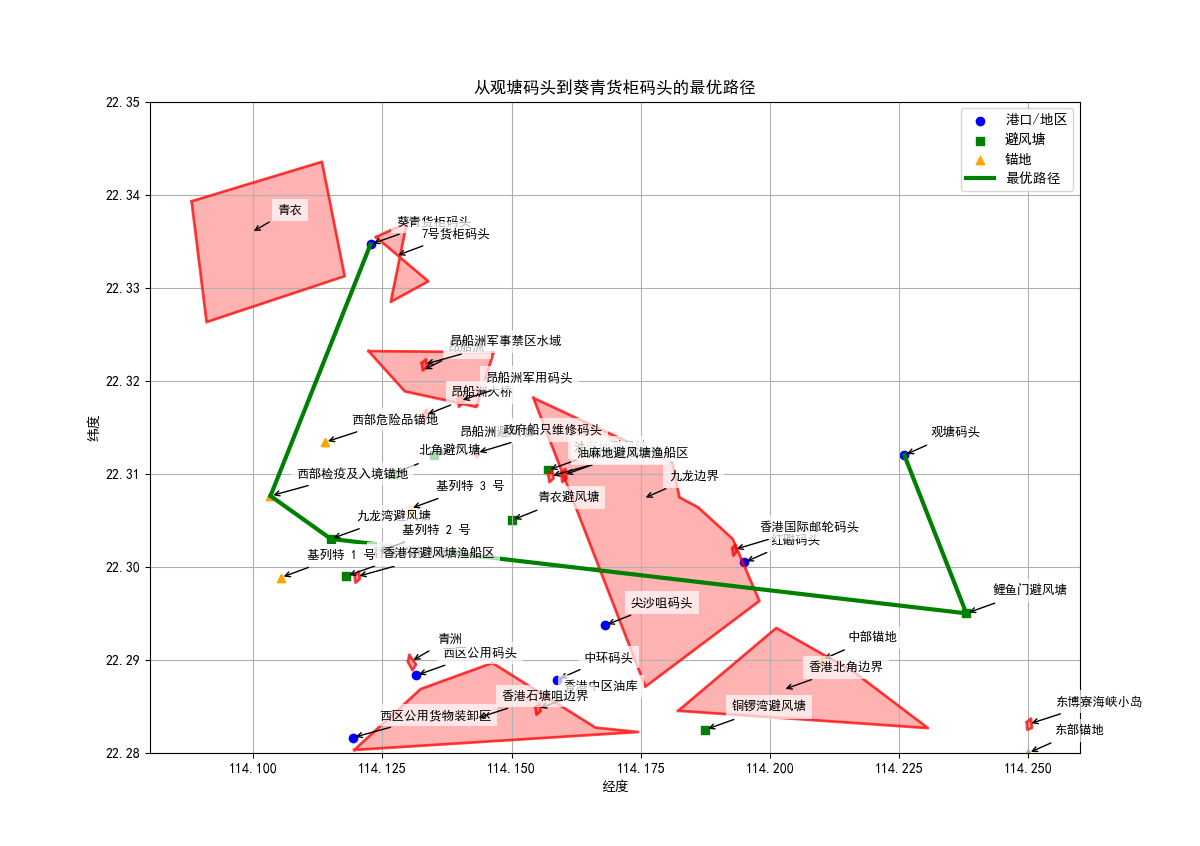
\includegraphics[width=0.8\textwidth]{Image/MD-Astar_BestPath.png}
    \captionof{figure}{5 从观塘码头到葵青货柜码头的最优路径(论文图4.3)}
\end{center}
\end{frame}

% 第5页:启发式函数可视化
\begin{frame}[plain]{启发式函数可视化展示}
\begin{center}
    \includegraphics[width=0.8\textwidth]{Image/MD-Astar_Heuristic.png}
    \captionof{figure}{6 启发式函数权重分布可视化(论文图4.1)}
\end{center}
\end{frame}

% 第6页:AN-MPC 控制器轨迹仿真实验
\begin{frame}{AN-MPC控制器轨迹仿真}
\justifying
控制模块采用 AN-MPC 策略进行轨迹优化与扰动补偿。

\vspace{0.5em}
\textbf{实验设置:}
\begin{itemize}
    \item 引入水流扰动,方向与速度随机扰动;
    \item 采用参考路径点进行滚动优化控制;
    \item 实验中提前 128s 到达终点,成功触发终止机制。
\end{itemize}
\end{frame}

% 第7页:控制器实验轨迹图展示
\begin{frame}[plain]{AN-MPC轨迹仿真图示}
\begin{center}
    \includegraphics[height=0.7\textwidth]{Image/AN-MPC_Result.png}
    \captionof{figure}{7 含水流扰动条件下的 MPC 路径跟踪结果(论文图4.4)}
\end{center}
\end{frame}

\section{研究总结与展望}

% 第1页:研究总结与未来工作
\begin{frame}{研究总结与未来工作}
\justifying
本研究构建了一个面向水面无人艇(USV)的三层路径规划与控制框架,涵盖:

\begin{itemize}
    \item MD-A* 全局路径规划:结合欧几里得距离与绕行代价的启发式设计;
    \item AN-MPC 局部轨迹控制:基于 Fossen 模型实现动态误差调节与扰动补偿;
\end{itemize}

\vspace{0.5em}
\textbf{后续工作展望:}
\begin{itemize}
    \item 引入多智能体强化学习(MASAC),提升动态障碍规避与协同能力;
    \item 构建强化学习-AN-MPC–MD-A* 联动机制,实现路径规划与控制策略的融合调度;
    \item 拓展系统至真实海洋任务部署,探索稳定性与鲁棒性进一步提升路径。
\end{itemize}
\end{frame}

% 第2页:项目仓库链接(附录B3)
\begin{frame}{项目仓库链接说明}
\justifying
为提升本课题的可复现性与模块化可维护性,作者已将路径规划与控制器模块整理上传至 GitHub,涵盖核心代码、地图数据与实验图像。

\vspace{0.8em}
\textbf{项目地址:}
\begin{center}
\texttt{https://github.com/CGMgit/USV-MD-Astar-ANMPC}
\end{center}

\vspace{0.5em}
\textbf{仓库内容包括:}
\begin{itemize}
    \item \texttt{code/}:MD-A* 与 AN-MPC 实现代码;
    \item \texttt{data/}:仿真地图、节点点位与障碍数据;
    \item \texttt{figures/}:论文与答辩所用实验图;
    \item \texttt{README.md}:项目说明与复现指南。
\end{itemize}

\vspace{0.5em}
项目将在答辩结束后正式开源,欢迎交流与合作。
\end{frame}

\end{document}
